\begin{enumerate}
	\item Exercício
	
	\begin{equation*}
		0 \leq r \leq 3,\, 0 \leq \theta \leq \dfrac{\pi}{2},\, 0 \leq z \leq 2
	\end{equation*}
	
	\begin{figure}[htb]
		\caption{Coordenadas cilíndricas - Aula 03 - Exercício I}
		\label{v27_a03_e01}
		\centering
		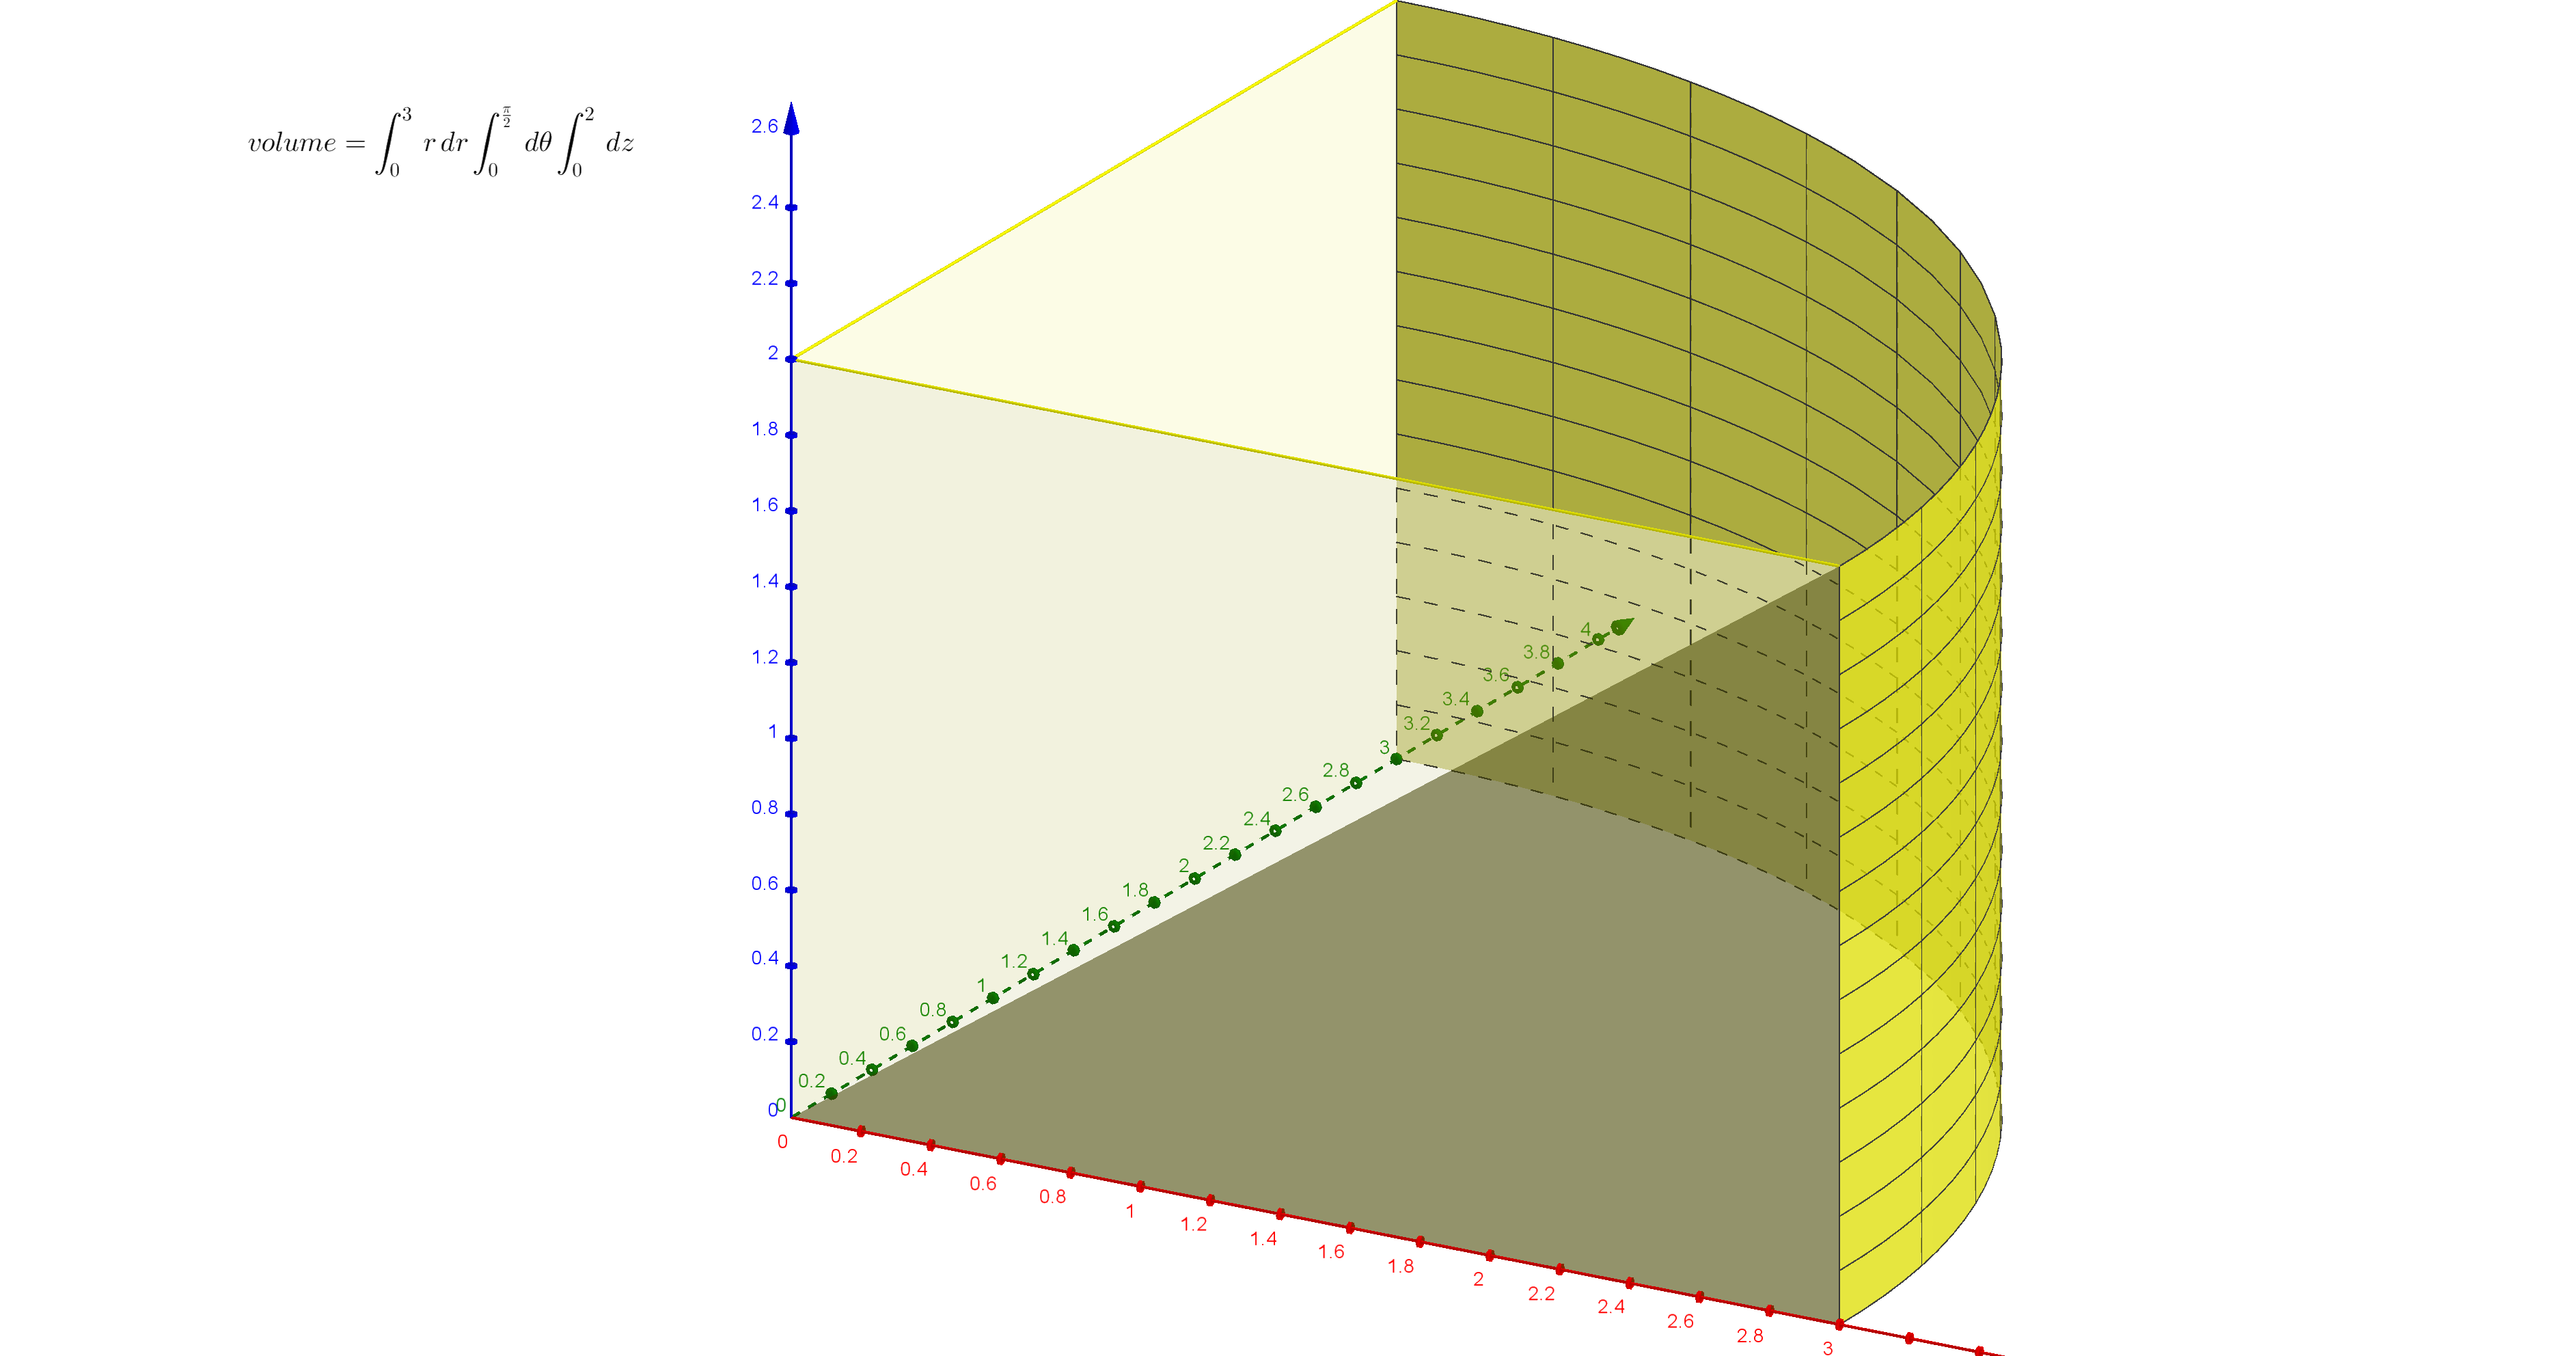
\includegraphics[width=0.5\textwidth]{v27_a03_e01.png}		
	\end{figure}
	
	\begin{gather*}
		\int_0^3 \int_0^{\frac{\pi}{2}} \int_0^2 r\, dz d\theta dr = \int_0^3 r\, dr \int_0^{\frac{\pi}{2}} d\theta \int_0^2 dz = \left[\dfrac{r^2}{2}\right]_0^3 \left[\theta\right]_0^{\frac{\pi}{2}} \left[z\right]_0^2 = \dfrac{9}{2}\dfrac{\pi}{\overstrike{2}}\overstrike{2} = \dfrac{9\pi}{2}
	\end{gather*}
\end{enumerate}